\documentclass[12pt, t]{beamer}
\usepackage{amsmath}
\usepackage{bm}
\usepackage{setspace}
\usepackage[style=phys, backend=biber]{biblatex}
\usepackage[no-math]{luatexja-fontspec}
\usepackage[utf8]{inputenc}
\usepackage{bxcoloremoji}
\usepackage{comment}
\addbibresource{all.bib}

% 論文タイトルの大文字小文字は bib ファイルのままにする
\DeclareFieldFormat{titlecase}{#1}

\setmainjfont{SourceHanSerifJP}
\setsansjfont{SourceHanSansJP}
\ltjsetparameter{jacharrange={-2}}

\renewcommand{\kanjifamilydefault}{\gtdefault}

\setstretch{1.1}
\setlength{\parskip}{7pt}

\usetheme{CambridgeUS}
\usefonttheme{professionalfonts}

\usepackage{geometry}
\usepackage{tikz}
\usetikzlibrary{calc, decorations.pathmorphing, patterns}
\usetikzlibrary{cd}
\usepackage[nomessages]{fp}

%%%%%%% 調和振動子系
%%%% \A*cos(\OMEGA*\t)+\B*sin(1.73*\OMEGA*\t) のパラメータ
\def\A{1}
\def\B{0.8}
\def\OMEGA{0.2}

%%% 壁などの描画のパラメータ
\def\wallHeight{2}
\def\wallWidth{0.2}
\def\totalLength{10}
\def\springStraightLength{0.2}
\def\axisDepth{-0.7}
%\def\t{27}

%%% 壁などのスタイル
\tikzset{wall/.style={pattern = north east lines}}
\tikzset{ball/.style={circle,shade,outer color=black!90!white,inner color=white,inner sep=2.5mm,label={$m$}}}
\tikzset{spring/.style={decorate,decoration={aspect=0.4, segment length=#1, amplitude=2mm,coil}}}
\tikzset{springk/.style={label={$k$},yshift=2}}

%%%%%%%

\newcommand{\eapple}{\coloremoji{🍎}}
\newcommand{\etangerine}{\coloremoji{🍊}}
\newcommand{\ebanana}{\coloremoji{🍌}}

\newcommand{\lr}[1]{\left({}#1\right){}}
\newcommand{\slr}[1]{\left[{}#1\right]{}}
\newcommand{\clr}[1]{\left\{{}#1\right\}{}}

\newcommand{\eAEB}{\slr{\eapple{}\etangerine{}\ebanana{}}}
\newcommand{\eABE}{\slr{\eapple{}\ebanana{}\etangerine{}}}
\newcommand{\eEAB}{\slr{\etangerine{}\eapple{}\ebanana{}}}
\newcommand{\eEBA}{\slr{\etangerine{}\ebanana{}\eapple{}}}
\newcommand{\eBAE}{\slr{\ebanana{}\eapple{}\etangerine{}}}
\newcommand{\eBEA}{\slr{\ebanana{}\etangerine{}\eapple{}}}

\def\opcty{0.1}

\title{群論という視点}
\author{武智}
\begin{document}
\frame{\maketitle}

\begin{frame}
\frametitle{はじめに}
現代数学では、ほとんど至るところで群論が使われている。

物理学でも使われているが、群論の言葉を明示的には使わずに議論を進めることも多い(当社比)。

情報科学では、暗号理論など一部を除いて、あからさまに群論が使われることは少ない(個人の感想です)。
\end{frame}

\begin{frame}
\frametitle{はじめに}
Q. 場の理論、楕円暗号のような、高度に抽象化された場面でしか群論は使えないのだろうか?

$\rightsquigarrow$ A. そんなことはない。

群は色々なところに潜んでいる。ただ、シンプルな系では、群論を意識せずに問題が解けてしまうことが多いため、
その御利益に気付きにくい。
\end{frame}


\begin{frame}{流れ}
\begin{enumerate}
\item 群とは
\begin{enumerate}
\item 置換群
\item 群の作用
\end{enumerate}
\item 代数方程式の非可解性
\item 群論の応用:$2$質点連成振動子系
\item ポエム
\end{enumerate}
\end{frame}

\begin{frame}
\frametitle{群とは}
初めて群を定義したのはGalois(1832)。

群の定義には至っていないものの、先駆的な研究としてLagrange(1771)やAbel(1824), Ruffini(1799)がある。

\end{frame}

\begin{frame}
\frametitle{置換群}
Galoisが導入したのは今で言う置換群。

元々Galoisは「置換の集まり」の意味で``groupe de substitusions''と呼んでいた。
繰り返し言及するうちに、一般名詞 groupe が数学用語になっていったらしい。

Galoisが数学用語としての groupe の定義を書き下したのは、決闘前夜だったという\cite{Neumann2011}。
\end{frame}

\begin{frame}
\frametitle{置換}
\eapple{}と\etangerine{}と\ebanana{}の並び方は
\begin{align}
  \Omega = \clr{
  \slr{\eapple{}\etangerine{}\ebanana{}},
  \slr{\eapple{}\ebanana{}\etangerine{}},
  \slr{\etangerine{}\ebanana{}\eapple{}},
  \slr{\etangerine{}\eapple{}\ebanana{}},
  \slr{\ebanana{}\eapple{}\etangerine{}},
  \slr{\ebanana{}\etangerine{}\eapple{}}} \notag
\end{align}
の$6$通り。
\end{frame}

\begin{frame}[fragile]
\frametitle{並び方の間の変換}
並び方の間の変換を全て考える。$6^2 = 36$個。
\[
\begin{tikzcd}
&
\eAEB
 \arrow[loop, out=120, in=60, looseness=3]
 \arrow[r, leftrightarrow]
 \arrow[rrd, leftrightarrow]
 \arrow[rdd, leftrightarrow]
 \arrow[dd, leftrightarrow]
 \arrow[ld, leftrightarrow]
&
\eABE
 \arrow[loop, out=120, in=60, looseness=3]
 \arrow[rd, leftrightarrow]
 \arrow[dd, leftrightarrow]
 \arrow[ldd, leftrightarrow]
 \arrow[lld, leftrightarrow]
&
\\
\eEAB
 \arrow[loop, out=120, in=60, looseness=3]
 \arrow[rrr, leftrightarrow]
 \arrow[rrd, leftrightarrow]
 \arrow[rd, leftrightarrow]
&
&
&
\eBAE
 \arrow[loop, out=120, in=60, looseness=3]
 \arrow[ld, leftrightarrow]
 \arrow[lld, leftrightarrow]
\\
&
\eEBA
 \arrow[loop, out=240, in=300, looseness=3]
 \arrow[r, leftrightarrow]
&
\eBEA
 \arrow[loop, out=240, in=300, looseness=3]
& 
\end{tikzcd}
\]
$6$個の並び方それぞれから$6$本の矢印が生える。
\end{frame}

\begin{frame}[fragile]
\frametitle{$e$}
自分自身へ戻る変換(恒等変換)$6$本をまとめて$e$と書く。
\[
\begin{tikzcd}
&
\eAEB
 \arrow[loop, out=120, in=60, looseness=3]
 \arrow[r, leftrightarrow, opacity=\opcty]
 \arrow[rrd, leftrightarrow, opacity=\opcty]
 \arrow[rdd, leftrightarrow, opacity=\opcty]
 \arrow[dd, leftrightarrow, opacity=\opcty]
 \arrow[ld, leftrightarrow, opacity=\opcty]
&
\eABE
 \arrow[loop, out=120, in=60, looseness=3]
 \arrow[rd, leftrightarrow, opacity=\opcty]
 \arrow[dd, leftrightarrow, opacity=\opcty]
 \arrow[ldd, leftrightarrow, opacity=\opcty]
 \arrow[lld, leftrightarrow, opacity=\opcty]
&
\\
\eEAB
 \arrow[loop, out=120, in=60, looseness=3]
 \arrow[rrr, leftrightarrow, opacity=\opcty]
 \arrow[rrd, leftrightarrow, opacity=\opcty]
 \arrow[rd, leftrightarrow, opacity=\opcty]
&
&
&
\eBAE
 \arrow[loop, out=120, in=60, looseness=3]
 \arrow[ld, leftrightarrow, opacity=\opcty]
 \arrow[lld, leftrightarrow, opacity=\opcty]
\\
&
\eEBA
 \arrow[loop, out=240, in=300, looseness=3]
 \arrow[r, leftrightarrow, opacity=\opcty]
&
\eBEA
 \arrow[loop, out=240, in=300, looseness=3]
& 
\end{tikzcd}
\]
$e$は$\Omega \rightarrow \Omega$の全単射となる。
\end{frame}


\begin{frame}[fragile]
\frametitle{$\sigma_{12}$}
$1$番目と$2$番目を入れ替える変換 $\sigma_{12}$
\[
\begin{tikzcd}
&
\eAEB
 \arrow[loop, out=120, in=60, looseness=3, opacity=\opcty]
 \arrow[r, leftrightarrow, opacity=\opcty]
 \arrow[rrd, leftrightarrow, opacity=\opcty]
 \arrow[rdd, leftrightarrow, opacity=\opcty]
 \arrow[dd, leftrightarrow, opacity=\opcty]
 \arrow[ld, leftrightarrow]
&
\eABE
 \arrow[loop, out=120, in=60, looseness=3, opacity=\opcty]
 \arrow[rd, leftrightarrow]
 \arrow[dd, leftrightarrow, opacity=\opcty]
 \arrow[ldd, leftrightarrow, opacity=\opcty]
 \arrow[lld, leftrightarrow, opacity=\opcty]
&
\\
\eEAB
 \arrow[loop, out=120, in=60, looseness=3, opacity=\opcty]
 \arrow[rrr, leftrightarrow, opacity=\opcty]
 \arrow[rrd, leftrightarrow, opacity=\opcty]
 \arrow[rd, leftrightarrow, opacity=\opcty]
&
&
&
\eBAE
 \arrow[loop, out=120, in=60, looseness=3, opacity=\opcty]
 \arrow[ld, leftrightarrow, opacity=\opcty]
 \arrow[lld, leftrightarrow, opacity=\opcty]
\\
&
\eEBA
 \arrow[loop, out=240, in=300, looseness=3, opacity=\opcty]
 \arrow[r, leftrightarrow]
&
\eBEA
 \arrow[loop, out=240, in=300, looseness=3, opacity=\opcty]
& 
\end{tikzcd}
\]
\end{frame}

\begin{frame}[fragile]
\frametitle{$\sigma_{23}$}
$2$番目と$3$番目を入れ替える変換 $\sigma_{23}$
\[
\begin{tikzcd}
&
\eAEB
 \arrow[loop, out=120, in=60, looseness=3, opacity=\opcty]
 \arrow[r, leftrightarrow]
 \arrow[rrd, leftrightarrow, opacity=\opcty]
 \arrow[rdd, leftrightarrow, opacity=\opcty]
 \arrow[dd, leftrightarrow, opacity=\opcty]
 \arrow[ld, leftrightarrow, opacity=\opcty]
&
\eABE
 \arrow[loop, out=120, in=60, looseness=3, opacity=\opcty]
 \arrow[rd, leftrightarrow, opacity=\opcty]
 \arrow[dd, leftrightarrow, opacity=\opcty]
 \arrow[ldd, leftrightarrow, opacity=\opcty]
 \arrow[lld, leftrightarrow, opacity=\opcty]
&
\\
\eEAB
 \arrow[loop, out=120, in=60, looseness=3, opacity=\opcty]
 \arrow[rrr, leftrightarrow, opacity=\opcty]
 \arrow[rrd, leftrightarrow, opacity=\opcty]
 \arrow[rd, leftrightarrow]
&
&
&
\eBAE
 \arrow[loop, out=120, in=60, looseness=3, opacity=\opcty]
 \arrow[ld, leftrightarrow]
 \arrow[lld, leftrightarrow, opacity=\opcty]
\\
&
\eEBA
 \arrow[loop, out=240, in=300, looseness=3, opacity=\opcty]
 \arrow[r, leftrightarrow, opacity=\opcty]
&
\eBEA
 \arrow[loop, out=240, in=300, looseness=3, opacity=\opcty]
& 
\end{tikzcd}
\]
\end{frame}

\begin{frame}[fragile]
\frametitle{$\sigma_{31}$}
$3$番目と$1$番目を入れ替える変換 $\sigma_{31}$
\[
\begin{tikzcd}
&
\eAEB
 \arrow[loop, out=120, in=60, looseness=3, opacity=\opcty]
 \arrow[r, leftrightarrow, opacity=\opcty]
 \arrow[rrd, leftrightarrow, opacity=\opcty]
 \arrow[rdd, leftrightarrow]
 \arrow[dd, leftrightarrow, opacity=\opcty]
 \arrow[ld, leftrightarrow, opacity=\opcty]
&
\eABE
 \arrow[loop, out=120, in=60, looseness=3, opacity=\opcty]
 \arrow[rd, leftrightarrow, opacity=\opcty]
 \arrow[dd, leftrightarrow, opacity=\opcty]
 \arrow[ldd, leftrightarrow]
 \arrow[lld, leftrightarrow, opacity=\opcty]
&
\\
\eEAB
 \arrow[loop, out=120, in=60, looseness=3, opacity=\opcty]
 \arrow[rrr, leftrightarrow]
 \arrow[rrd, leftrightarrow, opacity=\opcty]
 \arrow[rd, leftrightarrow, opacity=\opcty]
&
&
&
\eBAE
 \arrow[loop, out=120, in=60, looseness=3, opacity=\opcty]
 \arrow[ld, leftrightarrow, opacity=\opcty]
 \arrow[lld, leftrightarrow, opacity=\opcty]
\\
&
\eEBA
 \arrow[loop, out=240, in=300, looseness=3, opacity=\opcty]
 \arrow[r, leftrightarrow, opacity=\opcty]
&
\eBEA
 \arrow[loop, out=240, in=300, looseness=3, opacity=\opcty]
& 
\end{tikzcd}
\]
\end{frame}

\begin{frame}[fragile]
\frametitle{$\sigma_{123}$}
$1$番目$\rightarrow$$2$番目$\rightarrow$$3$番目$\rightarrow$$1$番目と入れ替える変換 $\sigma_{123}$
\[
\begin{tikzcd}
&
\eAEB
 \arrow[loop, out=120, in=60, looseness=3, opacity=\opcty]
 \arrow[r, leftrightarrow, opacity=\opcty]
 \arrow[rrd, rightarrow]
 \arrow[rrd, leftrightarrow, opacity=\opcty]
 \arrow[rdd, leftrightarrow, opacity=\opcty]
 \arrow[dd, leftrightarrow, opacity=\opcty]
 \arrow[ld, leftrightarrow, opacity=\opcty]
&
\eABE
 \arrow[loop, out=120, in=60, looseness=3, opacity=\opcty]
 \arrow[rd, leftrightarrow, opacity=\opcty]
 \arrow[dd, leftrightarrow, opacity=\opcty]
 \arrow[ldd, leftrightarrow, opacity=\opcty]
 \arrow[lld, rightarrow]
 \arrow[lld, leftrightarrow, opacity=\opcty]
&
\\
\eEAB
 \arrow[loop, out=120, in=60, looseness=3, opacity=\opcty]
 \arrow[rrr, leftrightarrow, opacity=\opcty]
 \arrow[rrd, rightarrow]
 \arrow[rrd, leftrightarrow, opacity=\opcty]
 \arrow[rd, leftrightarrow, opacity=\opcty]
&
&
&
\eBAE
 \arrow[loop, out=120, in=60, looseness=3, opacity=\opcty]
 \arrow[ld, leftrightarrow, opacity=\opcty]
 \arrow[lld, rightarrow]
 \arrow[lld, leftrightarrow, opacity=\opcty]
\\
&
\eEBA
 \arrow[loop, out=240, in=300, looseness=3, opacity=\opcty]
 \arrow[r, leftrightarrow, opacity=\opcty]
 \arrow[uu, rightarrow]
&
\eBEA
 \arrow[loop, out=240, in=300, looseness=3, opacity=\opcty]
 \arrow[uu, rightarrow]
& 
\end{tikzcd}
\]
\end{frame}

\begin{frame}[fragile]
\frametitle{$\sigma_{321}$}
$3$番目$\rightarrow$$2$番目$\rightarrow$$1$番目$\rightarrow$$3$番目と入れ替える変換 $\sigma_{321}$
\[
\begin{tikzcd}
&
\eAEB
 \arrow[loop, out=120, in=60, looseness=3, opacity=\opcty]
 \arrow[r, leftrightarrow, opacity=\opcty]
 \arrow[rrd, leftarrow]
 \arrow[rrd, leftrightarrow, opacity=\opcty]
 \arrow[rdd, leftrightarrow, opacity=\opcty]
 \arrow[dd, leftrightarrow, opacity=\opcty]
 \arrow[ld, leftrightarrow, opacity=\opcty]
&
\eABE
 \arrow[loop, out=120, in=60, looseness=3, opacity=\opcty]
 \arrow[rd, leftrightarrow, opacity=\opcty]
 \arrow[dd, leftrightarrow, opacity=\opcty]
 \arrow[ldd, leftrightarrow, opacity=\opcty]
 \arrow[lld, leftarrow]
 \arrow[lld, leftrightarrow, opacity=\opcty]
&
\\
\eEAB
 \arrow[loop, out=120, in=60, looseness=3, opacity=\opcty]
 \arrow[rrr, leftrightarrow, opacity=\opcty]
 \arrow[rrd, leftarrow]
 \arrow[rrd, leftrightarrow, opacity=\opcty]
 \arrow[rd, leftrightarrow, opacity=\opcty]
&
&
&
\eBAE
 \arrow[loop, out=120, in=60, looseness=3, opacity=\opcty]
 \arrow[ld, leftrightarrow, opacity=\opcty]
 \arrow[lld, leftarrow]
 \arrow[lld, leftrightarrow, opacity=\opcty]
\\
&
\eEBA
 \arrow[loop, out=240, in=300, looseness=3, opacity=\opcty]
 \arrow[r, leftrightarrow, opacity=\opcty]
 \arrow[uu, leftarrow]
&
\eBEA
 \arrow[loop, out=240, in=300, looseness=3, opacity=\opcty]
 \arrow[uu, leftarrow]
& 
\end{tikzcd}
\]
\end{frame}

\begin{frame}
\frametitle{変換の間の関係}
この$6$種類の変換をまとめて$S_3$と書く。
\begin{align}
  S_3 = \clr{e, \sigma_{12}, \sigma_{23}, \sigma_{31}, \sigma_{123}, \sigma_{321}}
\end{align}
$S_3$の元は$\Omega \rightarrow \Omega$の写像なので、合成写像を考えることができる。

例えば
$e(\sigma_{12}(\Omega)) = \sigma_{12}(\Omega)$なので$e$と$\sigma_{12}$の合成写像は$\sigma_{12}$.
\end{frame}

\begin{frame}[fragile]
\frametitle{$\sigma_{12} \cdot \sigma_{123} = \sigma_{23}$}
${\color{blue} \sigma_{12}}(\sigma_{123}(\Omega)) = {\color{red} \sigma_{23}}(\Omega)$
\[
\begin{tikzcd}
&
\eAEB
 \arrow[loop, out=120, in=60, looseness=3, opacity=\opcty]
 \arrow[r, leftrightarrow, red]
 \arrow[r, leftrightarrow, opacity=\opcty]
 \arrow[rrd, rightarrow]
 \arrow[rrd, leftrightarrow, opacity=\opcty]
 \arrow[rdd, leftrightarrow, opacity=\opcty]
 \arrow[dd, leftrightarrow, opacity=\opcty]
 \arrow[ld, leftrightarrow, blue]
&
\eABE
 \arrow[loop, out=120, in=60, looseness=3, opacity=\opcty]
 \arrow[rd, leftrightarrow, blue]
 \arrow[dd, leftrightarrow, opacity=\opcty]
 \arrow[ldd, leftrightarrow, opacity=\opcty]
 \arrow[lld, rightarrow]
 \arrow[lld, leftrightarrow, opacity=\opcty]
&
\\
\eEAB
 \arrow[loop, out=120, in=60, looseness=3, opacity=\opcty]
 \arrow[rrr, leftrightarrow, opacity=\opcty]
 \arrow[rrd, rightarrow]
 \arrow[rrd, leftrightarrow, opacity=\opcty]
 \arrow[rd, leftrightarrow, red]
&
&
&
\eBAE
 \arrow[loop, out=120, in=60, looseness=3, opacity=\opcty]
 \arrow[ld, leftrightarrow, red]
 \arrow[lld, rightarrow]
 \arrow[lld, leftrightarrow, opacity=\opcty]
\\
&
\eEBA
 \arrow[loop, out=240, in=300, looseness=3, opacity=\opcty]
 \arrow[r, leftrightarrow, blue]
 \arrow[uu, rightarrow]
&
\eBEA
 \arrow[loop, out=240, in=300, looseness=3, opacity=\opcty]
 \arrow[uu, rightarrow]
& 
\end{tikzcd}
\]
\end{frame}

\begin{frame}[fragile]
\frametitle{$\sigma_{31} \cdot \sigma_{12} = \sigma_{123}$}
${\color{blue} \sigma_{31}}(\sigma_{12}(\Omega)) = {\color{red} \sigma_{123}}(\Omega)$
\[
\begin{tikzcd}
&
\eAEB
 \arrow[loop, out=120, in=60, looseness=3, opacity=\opcty]
 \arrow[r, leftrightarrow, opacity=\opcty]
 \arrow[r, leftrightarrow, opacity=\opcty]
 \arrow[rrd, rightarrow, red]
 \arrow[rrd, leftrightarrow, opacity=\opcty]
 \arrow[rdd, leftrightarrow, blue]
 \arrow[dd, leftrightarrow, opacity=\opcty]
 \arrow[ld, leftrightarrow]
&
\eABE
 \arrow[loop, out=120, in=60, looseness=3, opacity=\opcty]
 \arrow[rd, leftrightarrow]
 \arrow[dd, leftrightarrow, opacity=\opcty]
 \arrow[ldd, leftrightarrow, blue]
 \arrow[lld, rightarrow, red]
 \arrow[lld, leftrightarrow, opacity=\opcty]
&
\\
\eEAB
 \arrow[loop, out=120, in=60, looseness=3, opacity=\opcty]
 \arrow[rrr, leftrightarrow, blue]
 \arrow[rrd, rightarrow, red]
 \arrow[rrd, leftrightarrow, opacity=\opcty]
 \arrow[rd, leftrightarrow, opacity=\opcty]
&
&
&
\eBAE
 \arrow[loop, out=120, in=60, looseness=3, opacity=\opcty]
 \arrow[ld, leftrightarrow, opacity=\opcty]
 \arrow[lld, rightarrow, red]
 \arrow[lld, leftrightarrow, opacity=\opcty]
\\
&
\eEBA
 \arrow[loop, out=240, in=300, looseness=3, opacity=\opcty]
 \arrow[r, leftrightarrow]
 \arrow[uu, rightarrow, red]
&
\eBEA
 \arrow[loop, out=240, in=300, looseness=3, opacity=\opcty]
 \arrow[uu, rightarrow, red]
& 
\end{tikzcd}
\]
\end{frame}

\begin{frame}
\frametitle{互換と、置換の偶奇}
$\sigma_{123}(\Omega) = \sigma_{12}(\sigma_{23}(\Omega)) = \sigma_{31}(\sigma_{12}(\Omega))$.

$\sigma_{12}$のような「$2$個の交換」を特に\alert{互換}と呼ぶ。
どんな並び方の変換(並び替え)も互換の組み合わせで書ける(cf. あみだくじ)。

並び替えを互換で表す組み合わせは色々あり得るが、互換個数の偶奇は変わらない。
\vspace{-1\zw}
\begin{center}
{\tiny
\begin{tabular}{cccccc}
&&&&& \\
\multicolumn{2}{c}{\eapple} & \multicolumn{2}{c}{\etangerine} & \multicolumn{2}{c}{\ebanana} \\
& \multicolumn{2}{|c|}{} & \multicolumn{2}{|c|}{} & \\
& \multicolumn{2}{|c|}{} & \multicolumn{2}{|c|}{} & \\
& \multicolumn{2}{|c|}{} & \multicolumn{2}{|c|}{} & \\\cline{4-5}
& \multicolumn{2}{|c|}{} & \multicolumn{2}{|c|}{} & \\\cline{2-3}
& \multicolumn{2}{|c|}{} & \multicolumn{2}{|c|}{} & \\
\multicolumn{2}{c}{\ebanana} & \multicolumn{2}{c}{\eapple} & \multicolumn{2}{c}{\etangerine}
\end{tabular}
$=$
\begin{tabular}{cccccc}
&&&&& \\
\multicolumn{2}{c}{\eapple} & \multicolumn{2}{c}{\etangerine} & \multicolumn{2}{c}{\ebanana} \\
& \multicolumn{2}{|c|}{} & \multicolumn{2}{|c|}{} & \\\cline{2-3}
& \multicolumn{2}{|c|}{} & \multicolumn{2}{|c|}{} & \\\cline{2-3}
& \multicolumn{2}{|c|}{} & \multicolumn{2}{|c|}{} & \\\cline{4-5}
& \multicolumn{2}{|c|}{} & \multicolumn{2}{|c|}{} & \\\cline{2-3}
& \multicolumn{2}{|c|}{} & \multicolumn{2}{|c|}{} & \\
\multicolumn{2}{c}{\ebanana} & \multicolumn{2}{c}{\eapple} & \multicolumn{2}{c}{\etangerine}
\end{tabular}
}
\end{center}

互換の個数が偶数(奇数)になる置換を偶置換(奇置換)と呼ぶ。
\end{frame}


\begin{frame}
\frametitle{合成$=$積}
写像の合成を、積の演算とみなす。$\sigma(\sigma'(\Omega)) = (\sigma \cdot \sigma')(\Omega)$
\begin{center}
\begin{tabular}{c|cccccc}
  $\sigma \backslash \sigma'$ & $e$            & $\sigma_{12}$  & $\sigma_{23}$  & $\sigma_{31}$  & $\sigma_{123}$ & $\sigma_{321}$ \\ \hline
  $e$                         & $e$            & $\sigma_{12}$  & $\sigma_{23}$  & $\sigma_{31}$  & $\sigma_{123}$ & $\sigma_{321}$ \\
  $\sigma_{12}$               & $\sigma_{12}$  & $e$            & $\sigma_{123}$ & $\sigma_{321}$ & $\sigma_{23}$  & $\sigma_{31}$  \\
  $\sigma_{23}$               & $\sigma_{23}$  & $\sigma_{321}$ & $e$            & $\sigma_{123}$ & $\sigma_{31}$  & $\sigma_{12}$  \\
  $\sigma_{31}$               & $\sigma_{31}$  & $\sigma_{123}$ & $\sigma_{321}$ & $e$            & $\sigma_{12}$  & $\sigma_{23}$  \\
  $\sigma_{123}$              & $\sigma_{123}$ & $\sigma_{31}$  & $\sigma_{12}$  & $\sigma_{23}$  & $\sigma_{321}$ & $e$            \\
  $\sigma_{321}$              & $\sigma_{321}$ & $\sigma_{23}$  & $\sigma_{31}$  & $\sigma_{12}$  & $e$            & $\sigma_{123}$
\end{tabular}
\end{center}
この表だけあれば、並び方$\Omega$の写像であることを忘れて
$S_3$だけで計算ができる。$\rightsquigarrow$ $S_3$を改めて数学的対象と考える。$\rightsquigarrow$ 群
\end{frame}


\begin{frame}
\frametitle{群の定義}
空でない集合$G$に$2$項演算$\cdot$が定義されていて、次の$3$条件
\begin{enumerate}
\item 結合則:任意の$a, b, c \in G$について $(a \cdot b) \cdot c = a \cdot (b \cdot c)$となる。
\item 単位元の存在:任意の$g \in G$について $g \cdot e = e \cdot g = g$ となる元 $e \in G$が存在する。
\item 逆元の存在:任意の$g \in G$について$g \cdot g^{-1} = g^{-1} \cdot g = e$ となる元 $g^{-1} \in G$が$g$ごとに存在する。
\end{enumerate}
を満たすとき、$G$は群であると言う。

$S_3$が群であることを確認しよう。
\end{frame}

\begin{frame}[fragile]
\frametitle{結合則}
結合則は、$\sigma \in S_3$が写像なので自然に成立。
\[
\begin{tikzcd}
&
\eAEB
 \arrow[loop, out=120, in=60, looseness=3, opacity=\opcty]
 \arrow[r, leftrightarrow, opacity=\opcty]
 \arrow[rrd, leftrightarrow, opacity=\opcty]
 \arrow[rdd, leftrightarrow, opacity=\opcty]
 \arrow[dd, leftrightarrow, opacity=\opcty]
 \arrow[ld, leftrightarrow, opacity=\opcty]
 \arrow[ld, rightarrow]
&
\eABE
 \arrow[loop, out=120, in=60, looseness=3, opacity=\opcty]
 \arrow[rd, leftrightarrow, opacity=\opcty]
 \arrow[dd, leftrightarrow, opacity=\opcty]
 \arrow[ldd, leftrightarrow, opacity=\opcty]
 \arrow[lld, leftrightarrow, opacity=\opcty]
&
\\
\eEAB
 \arrow[loop, out=120, in=60, looseness=3, opacity=\opcty]
 \arrow[rrr, leftrightarrow, opacity=\opcty]
 \arrow[rrd, leftrightarrow, opacity=\opcty]
 \arrow[rd, leftrightarrow, opacity=\opcty]
 \arrow[rd, rightarrow, blue]
&
&
&
\eBAE
 \arrow[loop, out=120, in=60, looseness=3, opacity=\opcty]
 \arrow[ld, leftrightarrow, opacity=\opcty]
 \arrow[lld, leftrightarrow, opacity=\opcty]
\\
&
\eEBA
 \arrow[loop, out=240, in=300, looseness=3, opacity=\opcty]
 \arrow[r, leftrightarrow, opacity=\opcty]
 \arrow[ruu, rightarrow, red]
&
\eBEA
 \arrow[loop, out=240, in=300, looseness=3, opacity=\opcty]
& 
\end{tikzcd}
\]
${\color{red} \sigma_{31}} \cdot {\color{blue} \sigma_{23}} \cdot \sigma_{12}$
\end{frame}

\begin{frame}[fragile]
\frametitle{結合則}
結合則は、$\sigma \in S_3$が写像なので自然に成立。
\[
\begin{tikzcd}
&
\eAEB
 \arrow[loop, out=120, in=60, looseness=3, opacity=\opcty]
 \arrow[r, leftrightarrow, opacity=\opcty]
 \arrow[rrd, leftrightarrow, opacity=\opcty]
 \arrow[rdd, leftrightarrow, opacity=\opcty]
 \arrow[dd, leftrightarrow, opacity=\opcty]
 \arrow[ld, leftrightarrow, opacity=\opcty]
 \arrow[ld, rightarrow, opacity=0.1]
 \arrow[dd, rightarrow, green]
&
\eABE
 \arrow[loop, out=120, in=60, looseness=3, opacity=\opcty]
 \arrow[rd, leftrightarrow, opacity=\opcty]
 \arrow[dd, leftrightarrow, opacity=\opcty]
 \arrow[ldd, leftrightarrow, opacity=\opcty]
 \arrow[lld, leftrightarrow, opacity=\opcty]
&
\\
\eEAB
 \arrow[loop, out=120, in=60, looseness=3, opacity=\opcty]
 \arrow[rrr, leftrightarrow, opacity=\opcty]
 \arrow[rrd, leftrightarrow, opacity=\opcty]
 \arrow[rd, leftrightarrow, opacity=\opcty]
 \arrow[rd, rightarrow, blue, opacity=0.1]
&
&
&
\eBAE
 \arrow[loop, out=120, in=60, looseness=3, opacity=\opcty]
 \arrow[ld, leftrightarrow, opacity=\opcty]
 \arrow[lld, leftrightarrow, opacity=\opcty]
\\
&
\eEBA
 \arrow[loop, out=240, in=300, looseness=3, opacity=\opcty]
 \arrow[r, leftrightarrow, opacity=\opcty]
 \arrow[ruu, rightarrow, red]
&
\eBEA
 \arrow[loop, out=240, in=300, looseness=3, opacity=\opcty]
& 
\end{tikzcd}
\]
${\color{red} \sigma_{31}} \cdot {\color{blue} \sigma_{23}} \cdot \sigma_{12}
= {\color{red} \sigma_{31}} \cdot ({\color{blue} \sigma_{23}} \cdot \sigma_{12})
= {\color{red} \sigma_{31}} \cdot {\color{green} \sigma_{321}}$
\end{frame}

\begin{frame}[fragile]
\frametitle{結合則}
結合則は、$\sigma \in S_3$が写像なので自然に成立。
\[
\begin{tikzcd}
&
\eAEB
 \arrow[loop, out=120, in=60, looseness=3, opacity=\opcty]
 \arrow[r, leftrightarrow, opacity=\opcty]
 \arrow[rrd, leftrightarrow, opacity=\opcty]
 \arrow[rdd, leftrightarrow, opacity=\opcty]
 \arrow[dd, leftrightarrow, opacity=\opcty]
 \arrow[ld, leftrightarrow, opacity=\opcty]
 \arrow[ld, rightarrow]
&
\eABE
 \arrow[loop, out=120, in=60, looseness=3, opacity=\opcty]
 \arrow[rd, leftrightarrow, opacity=\opcty]
 \arrow[dd, leftrightarrow, opacity=\opcty]
 \arrow[ldd, leftrightarrow, opacity=\opcty]
 \arrow[lld, leftrightarrow, opacity=\opcty]
&
\\
\eEAB
 \arrow[loop, out=120, in=60, looseness=3, opacity=\opcty]
 \arrow[rrr, leftrightarrow, opacity=\opcty]
 \arrow[rrd, leftrightarrow, opacity=\opcty]
 \arrow[rd, leftrightarrow, opacity=\opcty]
 \arrow[rd, rightarrow, blue, opacity=0.1]
 \arrow[rru, rightarrow, purple]
&
&
&
\eBAE
 \arrow[loop, out=120, in=60, looseness=3, opacity=\opcty]
 \arrow[ld, leftrightarrow, opacity=\opcty]
 \arrow[lld, leftrightarrow, opacity=\opcty]
\\
&
\eEBA
 \arrow[loop, out=240, in=300, looseness=3, opacity=\opcty]
 \arrow[r, leftrightarrow, opacity=\opcty]
 \arrow[ruu, rightarrow, red, opacity=0.1]
&
\eBEA
 \arrow[loop, out=240, in=300, looseness=3, opacity=\opcty]
& 
\end{tikzcd}
\]
${\color{red} \sigma_{31}} \cdot {\color{blue} \sigma_{23}} \cdot \sigma_{12}
= ({\color{red} \sigma_{31}} \cdot {\color{blue} \sigma_{23}}) \cdot \sigma_{12}
= {\color{purple} \sigma_{321}} \cdot \sigma_{12}$
\end{frame}


\begin{frame}[fragile]
\frametitle{単位元}
単位元は恒等写像 $e$.
\[
\begin{tikzcd}
&
\eAEB
 \arrow[loop, out=120, in=60, looseness=3]
 \arrow[r, leftrightarrow, opacity=\opcty]
 \arrow[rrd, leftrightarrow, opacity=\opcty]
 \arrow[rdd, leftrightarrow, opacity=\opcty]
 \arrow[dd, leftrightarrow, opacity=\opcty]
 \arrow[ld, leftrightarrow, opacity=\opcty]
&
\eABE
 \arrow[loop, out=120, in=60, looseness=3]
 \arrow[rd, leftrightarrow, opacity=\opcty]
 \arrow[dd, leftrightarrow, opacity=\opcty]
 \arrow[ldd, leftrightarrow, opacity=\opcty]
 \arrow[lld, leftrightarrow, opacity=\opcty]
&
\\
\eEAB
 \arrow[loop, out=120, in=60, looseness=3]
 \arrow[rrr, leftrightarrow, opacity=\opcty]
 \arrow[rrd, leftrightarrow, opacity=\opcty]
 \arrow[rd, leftrightarrow, opacity=\opcty]
&
&
&
\eBAE
 \arrow[loop, out=120, in=60, looseness=3]
 \arrow[ld, leftrightarrow, opacity=\opcty]
 \arrow[lld, leftrightarrow, opacity=\opcty]
\\
&
\eEBA
 \arrow[loop, out=240, in=300, looseness=3]
 \arrow[r, leftrightarrow, opacity=\opcty]
&
\eBEA
 \arrow[loop, out=240, in=300, looseness=3]
& 
\end{tikzcd}
\]
\end{frame}

\begin{frame}[fragile]
\frametitle{逆元}
逆元も、$\sigma \in S_3$が写像(矢印)なので自然に存在。
\[
\begin{tikzcd}
&
\eAEB
 \arrow[loop, out=120, in=60, looseness=3]
 \arrow[r, leftrightarrow]
 \arrow[rrd, leftrightarrow]
 \arrow[rdd, leftrightarrow]
 \arrow[dd, leftrightarrow]
 \arrow[ld, leftrightarrow]
&
\eABE
 \arrow[loop, out=120, in=60, looseness=3]
 \arrow[rd, leftrightarrow]
 \arrow[dd, leftrightarrow]
 \arrow[ldd, leftrightarrow]
 \arrow[lld, leftrightarrow]
&
\\
\eEAB
 \arrow[loop, out=120, in=60, looseness=3]
 \arrow[rrr, leftrightarrow]
 \arrow[rrd, leftrightarrow]
 \arrow[rd, leftrightarrow]
&
&
&
\eBAE
 \arrow[loop, out=120, in=60, looseness=3]
 \arrow[ld, leftrightarrow]
 \arrow[lld, leftrightarrow]
\\
&
\eEBA
 \arrow[loop, out=240, in=300, looseness=3]
 \arrow[r, leftrightarrow]
&
\eBEA
 \arrow[loop, out=240, in=300, looseness=3]
& 
\end{tikzcd}
\]
$\therefore$ $S_3$は群。$S_3$は$3$次対称群と呼ばれる。
\end{frame}

\begin{frame}
\frametitle{自明な群}
最も簡単な群は、恒等変換$e$だけから成る群である。
\begin{enumerate}
\item 結合側:$(e \cdot e) \cdot e = e \cdot (e \cdot e)$
\item 単位元:$e \cdot e = e$
\item 逆元:$e \cdot e = e \Rightarrow e^{-1} = e$
\end{enumerate}
この$\clr{e}$を自明な群と呼ぶ。
\end{frame}

\begin{frame}
\frametitle{部分群}
ある群の部分集合だけで群になることがある。

例えば$S_3$の中で
\begin{align}
  \Sigma_{12} &= \clr{e,\ \sigma_{12}},\
  \Sigma_{23} = \clr{e,\ \sigma_{23}},\
  \Sigma_{31} = \clr{e,\ \Sigma_{31}},\\
  A_3 &= \clr{e,\ \sigma_{123},\ \sigma_{321}}
\end{align}
はそれぞれ群になる。\\このようなとき、$A_3$は$S_3$の部分群であると言う。
\end{frame}

\begin{frame}
\frametitle{$3$次交代群}
$A_3$は$S_3$の中の偶置換を集めたもの(偶置換同士の積は偶置換)。
\begin{center}
\begin{tabular}{c|ccc}
                 &$e$           &$\sigma_{123}$&$\sigma_{321}$\\ \hline
  $e$            &$e$           &$\sigma_{123}$&$\sigma_{321}$\\
  $\sigma_{123}$ &$\sigma_{123}$&$\sigma_{321}$&$e$ \\
  $\sigma_{321}$ &$\sigma_{321}$&$e$           &$\sigma_{123}$
\end{tabular}
\end{center}

一般に、$n$次対称群$S_n$($n$要素の置換全体のなす群)の中で、\\
偶置換全体のなす部分群$A_n$を$n$次交代群と呼ぶ。
%なお、構成要素が$3$個の群は必ず$A_3$と同じ(同型)になる。
\end{frame}

\begin{comment}

\begin{frame}
\frametitle{$3$次交代群}
互いに異なる元$3$個からなる群を$G_3$とする。
$G_3$の元のうち$1$つは単位元$e$なので$G_3 = \clr{e, g, h}$と書いておく。

積の表は、単位元の性質から
\begin{center}
\begin{tabular}{c|ccc}
      &$e$&$g$&$h$\\ \hline
  $e$ &$e$&$g$&$h$\\
  $g$ &$g$&   & \\
  $h$ &$h$&   &
\end{tabular}
\end{center}
\end{frame}

\begin{frame}
\frametitle{$3$次交代群}
$g \cdot h = g$とすると、$h = e$になってしまう。\\
$g \cdot h = h$とすると、$g = e$になってしまう。\\
したがって$g \cdot h = e$.同様に$h \cdot g = e$.
\begin{center}
\begin{tabular}{c|ccc}
      &$e$&$g$&$h$\\ \hline
  $e$ &$e$&$g$&$h$\\
  $g$ &$g$&   &$e$\\
  $h$ &$h$&$e$&
\end{tabular}
\end{center}
\end{frame}

\begin{frame}
\frametitle{$3$次交代群}
$g \cdot g = g$とすると、両辺に$g^{-1}$をかけると$g = e$になってしまう。
$g \cdot g = e$とすると、$g \cdot h = e$なので$g = h$になってしまう。\\
したがって$g \cdot g = h$.
同様に$h \cdot h = g$.
\begin{center}
\begin{tabular}{c|ccc}
      &$e$&$g$&$h$\\ \hline
  $e$ &$e$&$g$&$h$\\
  $g$ &$g$&$h$&$e$\\
  $h$ &$h$&$e$&$g$
\end{tabular}
$=$
\begin{tabular}{c|ccc}
                 &$e$           &$\sigma_{123}$&$\sigma_{321}$\\ \hline
  $e$            &$e$           &$\sigma_{123}$&$\sigma_{321}$\\
  $\sigma_{123}$ &$\sigma_{123}$&$\sigma_{321}$&$e$ \\
  $\sigma_{321}$ &$\sigma_{321}$&$e$           &$\sigma_{123}$
\end{tabular}
\end{center}
$3$元からなる群は常に$A_3$と同じ(同型)になる。
\end{frame}

\end{comment}

\begin{frame}
\frametitle{作用}
$S_3$は並べ方の集合$\Omega$上の変換を集めたものだった。
このようなとき、$S_3$は$\Omega$に\alert{作用する}という。

一般に、群$G (\ni g)$と集合$X (\ni x)$について写像$g(x) \in X$が存在し
\begin{enumerate}
\item $g(h(x)) = (g \cdot h)(x)$
\item $e(x) = x$
\end{enumerate}
が成立するとき、$G$は$X$に作用するという。

歴史的には、作用から群が抽出された(作用 $\rightarrow$ 群)。

現代数学では抽象的に群を導入し、それを色々な集合に作用させる
という使い方が多い(群 $\rightarrow$ 作用)。
\end{frame}

\begin{frame}
\frametitle{自分自身への作用}
$S_3$は並べ方($\eAEB$など)に作用する群だったが、
$S_3$を集合とみなせば、$S_3$は$S_3$自身に作用することができる。

自分自身への作用の仕方は無数にあるが、例えば
$\sigma_a, \sigma_b \in S_3$について $\sigma_a(\sigma_b) = \sigma_a \cdot \sigma_b \in S_3$と
とればよい。
\begin{enumerate}
\item $\sigma_a(\sigma_b(\sigma)) = \sigma_a \cdot \sigma_b \cdot \sigma = (\sigma_a \cdot \sigma_b)(\sigma)$
\item $e(\sigma) = e \cdot \sigma = \sigma$
\end{enumerate}
なので、これは作用になる。
\end{frame}

\begin{frame}[fragile]
\frametitle{自分自身への作用}
\[
\begin{tikzcd}
&
e
 \arrow[loop, out=120, in=60, looseness=3]
 \arrow[r, leftrightarrow]
 \arrow[rrd, leftrightarrow]
 \arrow[rdd, leftrightarrow]
 \arrow[dd, leftrightarrow]
 \arrow[ld, leftrightarrow]
&
\sigma_{23}
 \arrow[loop, out=120, in=60, looseness=3]
 \arrow[rd, leftrightarrow]
 \arrow[dd, leftrightarrow]
 \arrow[ldd, leftrightarrow]
 \arrow[lld, leftrightarrow]
&
\\
\sigma_{12}
 \arrow[loop, out=120, in=60, looseness=3]
 \arrow[rrr, leftrightarrow]
 \arrow[rrd, leftrightarrow]
 \arrow[rd, leftrightarrow]
&
&
&
\sigma_{123}
 \arrow[loop, out=120, in=60, looseness=3]
 \arrow[ld, leftrightarrow]
 \arrow[lld, leftrightarrow]
\\
&
\sigma_{321}
 \arrow[loop, out=240, in=300, looseness=3]
 \arrow[r, leftrightarrow]
&
\sigma_{31}
 \arrow[loop, out=240, in=300, looseness=3]
& 
\end{tikzcd}
\]
\end{frame}

\begin{frame}
\frametitle{整数}
自分自身への作用の例として、整数$\mathbb{Z}$がある。

整数$\mathbb{Z}$は加法$+$について$0$を単位元とする群である。
\begin{enumerate}
\item $(k + l) + m = k + (l + m)$
\item $k + 0 = 0 + k = k$
\item $k + (-k) = (-k) + k = 0$
\end{enumerate}

$3 + 4 = 7$は、
「$3$を足す」と「$4$を足す」の合成が「$7$を足す」になる、と考えることもできるし、
「整数$3$」に「$4$を足す」を作用させると「整数$7$」になる、と考えることもできる。
\end{frame}

\begin{frame}
\frametitle{対称性}
群は対称性を記述する道具であると言われる。

集合$X$上のある全単射 $f: X \rightarrow X; x \mapsto f(x)$について、
\begin{align}
  f(\xi) = \xi
\end{align}
が成立するとき、$\xi$は\alert{$f$不変である}、または\alert{$f$対称である}と言う。
\end{frame}

\begin{frame}
\frametitle{対称性と群}
$\xi \in X$について、$f(\xi) = \xi$となる変換$f$の全体を$F$とすると、\\
$F$は$f(g(\xi)) = (f \cdot g)(\xi)$を積演算として群になる。

\begin{enumerate}
\item 結合則:$((f \cdot g) \cdot h)(\xi) = f(g(h(\xi))) = (f \cdot (g \cdot h))(\xi)$
\item 単位元:恒等変換 $e(\xi) = \xi$ なので $e \in F$
\item 逆元:$f^{-1}(f(\xi)) = f^{-1}(\xi) = \xi$なので$f^{-1} \in F$
\end{enumerate}

このようにして、対称性(不変性)と群が対応する。
\end{frame}


\begin{frame}
\frametitle{Abel-Ruffiniの定理}
$5$次以上の方程式は解の公式を持たない。

その証明に、なぜ群が必要だったのか。

真面目にやると$1$学期かかるので、「気分」だけを簡単に。
\end{frame}

\begin{frame}
\frametitle{$2$次方程式}
$2$次方程式 $x^2 + bx + c = 0$ を考える。$b, c$は有理数とする。\\
$2$つの解を $\alpha, \beta$ とおくと
\begin{align}
  x^2 + bx + c &= (x - \alpha)(x - \beta) \notag \\
  &= x^2 -(\alpha + \beta)x + \alpha \beta
\end{align}
より、
\begin{align}
  b &= -(\alpha + \beta) \\
  c &= \alpha \beta
\end{align}
を得る。
\end{frame}

\begin{frame}
\frametitle{置換に対する対称性}
$b = -(\alpha + \beta),\ c = \alpha \beta$は、$\alpha \leftrightarrow \beta$の置換について不変。\\
つまり、$\alpha$と$\beta$の互換を$\sigma_{\alpha \beta}$と書くと、
\begin{align}
  \sigma_{\alpha \beta}(b) &= \sigma_{\alpha \beta} (-(\alpha + \beta)) \notag \\
                           &= -(\beta + \alpha) = b \\
  \sigma_{\alpha \beta}(c) &= \sigma_{\alpha \beta}(\alpha \beta) \notag \\
                           &= \beta \alpha = c
\end{align}
である。(置換群を、多項式に作用させている)

また、$b,\ c$に四則演算を行った$b + c$や $c (b + 3 c/b)$なども、全て$\sigma_{\alpha \beta}$について不変。
\end{frame}

\begin{frame}
\frametitle{置換に対する対称性}
ところで、解$\alpha$そのものに$\sigma_{\alpha \beta}$を作用させると
\begin{align}
  \sigma_{\alpha \beta}(\alpha) = \beta \neq \alpha
\end{align}
すなわち$\alpha$は$\sigma_{\alpha \beta}$について不変ではない。$\beta$も同様。

$b,\ c$に四則演算を行ったものは全て$\sigma_{\alpha \beta}$について不変だったので、
\begin{center}
$\alpha$と$\beta$は $b,\ c$の四則演算だけで表すことはできない
\end{center}
ということが分かる。
\end{frame}

\begin{frame}
\frametitle{数の空間}
つまり、係数$b,\ c$の四則演算だけでは解$\alpha,\ \beta$に「到達」できない。\\
(四則演算だけで$2$次方程式の解の公式は得られない)
\[
\begin{tikzpicture}
\draw (-0.3,-0.15) node[anchor=south]{$b$};
\draw (0.3,-0.15) node[anchor=south]{$c$};
\draw (0,0) circle (1cm and 0.5cm);
\draw (0,-0.5) circle (1.75cm and 1cm);
\draw (0,-0.42) node[anchor=north]{{\small $b$と$c$の四則演算}};
\draw (0,-0.9) circle (2cm and 1.4cm);
\draw (-0.7,-1.8) node{$\alpha$};
\draw (0.7,-1.8) node{$\beta$};
\draw[->] (2.4,-0.2) node[anchor=west]{$S_2 = \clr{e,\ \sigma_{\alpha \beta}}$不変} -- (1.75, -0.5);
\draw[->] (2.4,-0.8) node[anchor=west]{$e$不変($=$自明な不変性しかない)} -- (2, -0.9);
\end{tikzpicture}
\]
$S_2$不変な数の集合から「抜け出す」ための演算が\alert{根号$\sqrt{\ }$}である。
\end{frame}

\begin{frame}
\frametitle{対称性を破る}
$\alpha - \beta$ は$\sigma_{\alpha \beta}$をかけると$-1$倍になる(不変でない)
\begin{align}
  \sigma_{\alpha \beta} \lr{\alpha - \beta} &= \beta - \alpha = -(\alpha - \beta)
\end{align}
しかし、その$2$乗である$(\alpha - \beta)^2$は、$(-1)^2 = 1$なので、
\begin{align}
  \sigma_{\alpha \beta} \lr{\lr{\alpha - \beta}^2} &= \lr{\sigma_{\alpha \beta}(\alpha - \beta)}^2 \notag \\
                                                   &= \clr{-\lr{\alpha - \beta}}^2 \notag \\
                                                   &= \lr{\alpha - \beta}^2
\end{align}
となり、$\sigma_{\alpha \beta}$不変になる。$\Leftrightarrow$ $b,\ c$で書ける。
\end{frame}

\begin{frame}
\frametitle{根号による対称性の減少}
すなわち、
\begin{align}
  (\alpha - \beta)^2 &= (\alpha + \beta)^2 - 4 \alpha \beta \notag \\
                     &= b^2 - 4 c \\
  \alpha - \beta &= \pm \sqrt{b^2 - 4 c}.
\end{align}
ここの根号$\pm \sqrt{\ }$で\alert{対称性が崩れる}。あとは、これと$\alpha + \beta = -b$を
連立すれば、$\alpha,\ \beta$が解ける。

$\rightsquigarrow$ $2$次方程式の解の公式が存在する。
\end{frame}

\begin{frame}
\frametitle{$3$次方程式}
$3$次方程式$x^3+bx^2+cx+d=0$についても、解を$\alpha,\ \beta,\ \gamma$として
\begin{align}
  b &= -(\alpha + \beta + \gamma) \\
  c &= \alpha \beta + \beta \gamma + \gamma \alpha \\
  d &= -\alpha \beta \gamma
\end{align}
であり、$b,\ c,\ d$は $\slr{\alpha \beta \gamma}$の置換$\sigma \in S_3$について不変。
\end{frame}

\begin{frame}
\frametitle{$3$次方程式の解の対称性}
解$\alpha,\ \beta,\ \gamma$は
$\alpha \rightarrow \beta \rightarrow \gamma \rightarrow \alpha$とする変換$\sigma_{\alpha \beta \gamma}$について
\begin{align}
  \sigma_{\alpha \beta \gamma}(\alpha) = \beta \neq \alpha
\end{align}
などとなり、$\alpha,\ \beta, \gamma$は$S_3$不変ではない。

$2$次方程式のときと同様、係数$b,\ c,\ d$の四則演算で解を記述することはできない。
\end{frame}

\begin{frame}
\frametitle{対称性の分解:$S_3 \rightarrow A_3$}
$2$次方程式における$\alpha - \beta$に対応するものが
\begin{align}
  T = (\alpha - \beta)(\beta - \gamma)(\gamma - \alpha)
\end{align}
である。$T$に奇置換$\clr{\sigma_{\alpha \beta}, \sigma_{\beta \gamma}, \sigma_{\gamma \alpha}}$をかけると$-1$倍になる。e.g.
\begin{align}
  \sigma_{\alpha \beta}(T) &= (\beta - \alpha)(\alpha - \gamma)(\gamma - \beta) = -(\alpha - \beta)(\beta - \gamma)(\gamma - \alpha) = -T \notag
\end{align}
一方、偶置換$\clr{e, \sigma_{\alpha \beta \gamma}, \sigma_{\gamma \beta \alpha}}$は
奇置換$2$個に分解できるので
\begin{align}
  \sigma_{\alpha \beta \gamma}(T) = \sigma_{\alpha \beta}(\sigma_{\beta \gamma}(T)) = (-1)^2 T = T
\end{align}
となり、$T$は偶置換で不変。
\end{frame}

\begin{frame}
\frametitle{対称性の分解:$S_3 \rightarrow A_3$}
$T$は奇置換で$-1$倍、偶置換で$1$倍(不変)であったので、
任意の置換$\sigma \in S_3$について、$T^2$は
\begin{align}
  \sigma(T^2) = (\sigma(T))^2 = (\pm T)^2 = T^2
\end{align}
となり、すなわち$S_3$不変。$\Leftrightarrow$ $T^2$は係数$b,\ c,\ d$で書ける。
\end{frame}

\begin{frame}
\frametitle{対称性の分解:$S_3 \rightarrow A_3$}
したがって、$T$は$b,\ c,\ d$と平方根$\sqrt{\ }$で記述できることになる。

しかし、$T$はまだ偶置換$\clr{e,\ \sigma_{\alpha \beta \gamma},\ \sigma_{\gamma \beta \alpha}}$で不変なので、
解$\alpha,\ \beta,\ \gamma$を$T$で記述することはできない。
\end{frame}

\begin{frame}
\frametitle{対称性の分解:$A_3 \rightarrow e$}
ここで、$1$の立方根$\omega_{\pm} = (-1 \pm \sqrt{-3})/2$を使って
\begin{align}
  U_{\pm} &= \alpha + \beta \omega_{\pm} + \gamma \omega_{\pm}^2
\end{align}
と置く。$U_{\pm}$に$\sigma_{\alpha \beta \gamma}$をかけると$\omega_{\mp}$倍になる。
\begin{align}
  \sigma_{\alpha \beta \gamma}\lr{U_{\pm}} &= \beta + \gamma \omega_{\pm} + \alpha \omega_{\pm}^2 \notag \\
                                     &= \omega_{\pm}^3 \lr{\beta + \gamma \omega_{\pm} + \alpha \omega_{\pm}^2} \notag \\
                                     &= \omega_{\pm}^2 \lr{\alpha + \beta \omega_{\pm} + \gamma \omega_{\pm}^2} = \omega_{\pm}^2 U = \omega_{\mp} U
\end{align}
なお、$\omega_\pm^3 = 1,\ \omega_\pm^2 = \omega_{\mp}$を使った。
\end{frame}

\begin{frame}
\frametitle{対称性の分解:$A_3 \rightarrow e$}
すると、$(\alpha - \beta)^2$や$T^2$と同じ仕組みで、
$U_{\pm}^3$は偶置換$\clr{\sigma_{\alpha \beta \gamma}, \sigma_{\gamma \beta \alpha}}$で不変になる。
\begin{align}
  \sigma_{\alpha \beta \gamma} \lr{U_{\pm}^3} &= (\omega_{\mp} U_{\pm})^3 = U_{\pm}^3 \\
  \sigma_{\gamma \beta \alpha} \lr{U_{\pm}^3} &= \lr{\sigma_{\alpha \beta \gamma}^2}\lr{U_{\pm}^3} = U_{\pm}^3
\end{align}
$U_{\pm}^3$は偶置換で不変。$\Leftrightarrow$ $U_{\pm}^3$は$T$を使えば記述できる。

$\Leftrightarrow$その立方根$U_{\pm}$は、$T$と立方根$\sqrt[3]{\ }$で記述できる。
\end{frame}

\begin{frame}
\frametitle{対称性の分解:$A_3 \rightarrow e$}
あとは、
\begin{align}
  -b   &= \alpha + \beta + \gamma \\
  U_+  &= \alpha + \beta \omega_+ + \gamma \omega_+^2 \\
  U_-  &= \alpha + \beta \omega_- + \gamma \omega_-^2
\end{align}
だったので、この$3$元連立方程式を解けば$\alpha,\ \beta,\ \gamma$が求められる。\\
$\rightsquigarrow$ 解が係数$b,\ c,\ d$と
$\sqrt{\ },\ \sqrt[3]{\ }$で記述される。\\
$\rightsquigarrow$ $3$次方程式の解の公式が存在する。
\end{frame}


\begin{frame}
\frametitle{数の空間}
\[
\begin{tikzpicture}
\draw (-0.3,-0.15) node[anchor=south]{$b$};
\draw (0,-0.15) node[anchor=south]{$c$};
\draw (0.3,-0.15) node[anchor=south]{$d$};
\draw (0,0) circle (1cm and 0.5cm);
\draw (0,-0.5) circle (1.75cm and 1cm);
\draw (0,-0.42) node[anchor=north]{{\tiny $b,c,d$の四則演算}};
\draw (0,-1.42) node[anchor=south]{$T^2$};
\draw (0,-0.9) circle (2cm and 1.4cm);
\draw (-0.7,-2.1) node[anchor=south]{$U_-^3$};
\draw (0.7,-2.1) node[anchor=south]{$U_+^3$};
\draw (0,-2.2) node[anchor=south]{$T$};
\draw (0,-1.3) circle (3cm and 1.8cm);
\draw (-1.2,-2.7) node[anchor=south]{$U_-$};
\draw (1.2,-2.7) node[anchor=south]{$U_+$};
\draw (-0.6,-2.8) node{$\alpha$};
\draw (0,-2.8) node{$\beta$};
\draw (0.6,-2.8) node{$\gamma$};
\draw[->] (3.4,0.0) node[anchor=west]{$S_3$不変} -- (1.75, -0.5);
\draw[->] (3.4,-0.6) node[anchor=west]{偶置換($A_3$)不変} -- (2, -0.9);
\draw[->] (3.4,-1.2) node[anchor=west]{$e$不変} -- (3, -1.3);
\end{tikzpicture}
\]
\end{frame}

\begin{frame}
\frametitle{$5$次方程式の非可解性}
\begin{center}
\begin{tabular}{c|cc}
                    &奇置換&偶置換 \\
                    &$\sigma_{\alpha \beta}$&$e$ \\ \hline
  係数$b,c$         &〇&〇 \\
  $(\alpha - \beta)^2$&〇&〇 \\
  $\alpha - \beta$  &$-1$倍&〇 \\
  解$\alpha, \beta$ &--&〇
\end{tabular}
\end{center}
\vspace{-1em}
$2$次方程式が解けたのは、
\begin{align}
\sigma_{\alpha \beta}(P^2) = P^2 \ \ \text{かつ} \ \ \sigma_{\alpha \beta}(P) \neq P
\end{align}
となる式$P = \alpha - \beta$が見付かったから。
\end{frame}

\begin{frame}
\frametitle{$5$次方程式の非可解性}
\begin{table}
\begin{tabular}{c|cccc}
       &奇置換                                & \multicolumn{2}{|c}{偶置換} \\
       &$\clr{\sigma_{\alpha \beta},\sigma_{\beta \gamma},\sigma_{\gamma \alpha}}$ & \multicolumn{1}{|c}{$\clr{\sigma_{\alpha \beta \gamma}, \sigma_{\gamma \beta \alpha}}$} & $e$ \\ \hline
  係数$b,c,d$&〇&〇&〇 \\
  $T^2$&〇&〇&〇 \\
  $T$  &$-1$倍&〇&〇 \\
  $U_{\pm}^3$ &--&〇&〇 \\
  $U_{\pm}$   &--&$\omega_{\mp}$倍&〇 \\
  解$\alpha, \beta,\gamma$ &--&--&〇
\end{tabular}
\end{table}
\vspace{-1em}
$3$次方程式が解けたのは、$e$でない偶置換$\sigma_\mathrm{ev} \in \clr{\sigma_{\alpha \beta \gamma}, \sigma_{\gamma \beta \alpha}}$で
\begin{align}
  \sigma_\mathrm{ev}(P^3) = P^3 \ \ \text{かつ} \ \ \sigma_\mathrm{ev}(P) \neq P
\end{align}
となる式$P = U_\pm$が見付かったから。
\end{frame}

\begin{frame}
\frametitle{$5$次方程式の非可解性}
解を$\clr{\alpha, \beta, \gamma, \delta, \eta}$とする$5$次方程式でも、$e$でない偶置換$\sigma_\mathrm{ev}$で
\begin{align}
  \sigma_\mathrm{ev}(P^3) = P^3 \ \ \text{かつ} \ \ \sigma_\mathrm{ev}(P) \neq P \label{eq:5cond}
\end{align}
となる式$P$を見付けなければならない。\\
しかし、$5$次の場合、$5$次巡回置換$\sigma_\mathrm{q}$(e.g. $\alpha \to$ $\beta \to$ $\gamma \to$ $\delta \to$ $\eta \to \alpha$)が
あり、任意の式$P$は$\sigma_{\mathrm{q}}^5(P) = P$となる。そして、
\begin{align}
  \clr{\sigma_{\mathrm{q}}^5(P) = P \ \ \text{かつ} \ \ \sigma_\mathrm{ev}(P^3) = P^3} \ \Rightarrow \ \sigma_\mathrm{ev}(P) = P
\end{align}
が証明できる。すなわち、(\ref{eq:5cond})の条件を満たす式$P$は存在しない。

$\rightsquigarrow$ $5$次方程式の解の公式は存在しない。
\end{frame}

\begin{frame}
\frametitle{対称性と空間}
実は、ここまでの議論でGalois理論は\alert{使っていない}。

Galois理論は、「数の空間$\leftrightarrow$対称性$\leftrightarrow$群」の対応を
より厳密かつスマートに記述する枠組みであり、今回は深入りしない。

ただ、Galois理論に言及せずとも、ここまでの議論で
\begin{center}
対称性で空間を分解する
\end{center}
という発想の一端は垣間見える。
そして、その裏には群の作用があることも分かる。
\end{frame}

\begin{frame}
\frametitle{空間の分解}
群論の発想は、具体的かつ実際的な問題にも応用できる。

最も分かりやすい例として調和振動子系を考える。
\end{frame}

\begin{frame}
\frametitle{固定端$2$質点連成振動}
質量$m$の$2$質点がばね係数$k$のばね$3$つで下図のように連結している。ばね両端は壁に固定。

\FPeval\t{27.0}%
\FPeval\u{\A*cos(\OMEGA*\t)+\B*sin(1.73*\OMEGA*\t)}%
\FPeval\v{\A*cos(\OMEGA*\t)-\B*sin(1.73*\OMEGA*\t)}%
{\centering
\begin{tikzpicture}[>=stealth]
%%% 左壁
\coordinate (south east of left wall) at (0,-.5*\wallHeight);
\coordinate (north west of left wall) at ($(south east of left wall) + (-\wallWidth,\wallHeight)$);
\fill[wall] (south east of left wall) rectangle (north west of left wall);
\draw[thick] (south east of left wall) -- (south east of left wall |- north west of left wall);
%%% 右壁
\coordinate (south west of right wall) at (\totalLength,-.5*\wallHeight);
\coordinate (north east of right wall) at ($(south west of right wall) + (\wallWidth,\wallHeight)$);
\fill[wall] (south west of right wall) rectangle (north east of right wall);
\draw[thick] (south west of right wall) -- (south west of right wall |- north east of right wall);
%%% おもり
\node[ball] (a) at (\totalLength/3 + \u,0) {};
\node[ball] (b) at (2*\totalLength/3 + \v,0) {};
%%% 座標軸
\draw[->] (0.5,\axisDepth) -- +(\totalLength-1,0);
\draw[dotted,thick] (\totalLength/3,\axisDepth-0.3) -- +(0,1.6)
              (2*\totalLength/3,\axisDepth-0.3) -- +(0,1.6)
              (a.south |- south east of left wall) -- (a.south)
              (b.south |- south east of left wall) -- (b.south);
\draw[->] (\totalLength/3,\axisDepth-0.15) --node[below] {$u_1$} +(\u,0);
\draw[->] (2*\totalLength/3,\axisDepth-0.15) --node[below] {$u_2$} +(\v,0);
%%% 座標計算
\coordinate (0) at (0,0);
\coordinate (0-right) at (\springStraightLength,0);
\coordinate (a-left) at ($(a.west) + (0.1-\springStraightLength,0)$);
\coordinate (a-right) at ($(a.east) + (\springStraightLength,0)$);
\coordinate (b-left) at ($(b.west) + (0.1-\springStraightLength,0)$);
\coordinate (b-right) at ($(b.east) + (\springStraightLength,0)$);
\coordinate (c-left) at (\totalLength + 0.1-\springStraightLength,0);
\coordinate (c) at (\totalLength,0);
%%% バネの直線部
\draw (0) -- (0-right)
      (a-left) -- (a.west)
      (a.east) -- (a-right)
      (b-left) -- (b.west)
      (b.east) -- (b-right)
      (c-left) -- (c);
%%% バネのグルグル部
\draw[spring={\totalLength/3 + \u}] (0-right) -- node[springk]{} (a-left);
\draw[spring={\totalLength/3 + \v - \u}] (a-right) -- node[springk]{} (b-left);
\draw[spring={\totalLength/3 - \v}] (b-right) -- node[springk]{} (c-left);
\end{tikzpicture}}

自然長(静止状態)からの変位を$u_i (i = 1,2)$とする。
\end{frame}

\begin{frame}
\frametitle{運動方程式}
$2$階の時間微分を$\ddot{u}$で表すと、運動方程式は
\begin{align}
  m \ddot{u}_1 &= -k u_1 + k (u_2 - u_1) \\
  m \ddot{u}_2 &= -k (u_2 - u_1) + k (-u_2)
\end{align}
すなわち
\begin{align}
  m \ddot{u}_1 &= -2k u_1 + k u_2 \\
  m \ddot{u}_2 &= k u_1 - 2k u_2
\end{align}
となる。
\end{frame}

\begin{frame}
\frametitle{運動方程式}
縦ベクトルで
\begin{align}
  \bm{u} = \lr{
  \begin{array}{c}
    u_1 \\
    u_2
  \end{array}}
\end{align}
とおくと、運動方程式は
\begin{align}
  \ddot{\bm{u}} &= \dfrac{k}{m} \lr{
  \begin{array}{cc}
    2 & -1 \\
    -1 & 2
  \end{array}} \bm{u} \\
  &= -\dfrac{k}{m} M \bm{u}
\end{align}
と書ける。
\end{frame}

\begin{frame}
\frametitle{通常の解法}
通常は、係数の行列$M$を対角化して解く。
\begin{align}
  M &= U^{-1} \bar{M} U \\
  U &= \dfrac{1}{\sqrt{2}}
  \lr{\begin{array}{cc}
        1 & 1 \\
        1 & -1
      \end{array}},\ 
  \bar{M} =
  \lr{\begin{array}{cc}
        1 & 0 \\
        0 & 3
      \end{array}} \\
\end{align}
\end{frame}

\begin{frame}
\frametitle{通常の解法}
\begin{align}
  \ddot{\bm{u}} = -\dfrac{k}{m} M \bm{u} \ \Leftrightarrow \ 
  U \ddot{\bm{u}} &= -\dfrac{k}{m} U U^{-1} \bar{M} U \bm{u} \notag \\
  U \ddot{\bm{u}} &= -\dfrac{k}{m} \bar{M} U \bm{u} \notag
\end{align}
ここで
\begin{align}
  \bm{v} = \lr{
  \begin{array}{c}
    v_1 \\
    v_2
  \end{array}} \equiv
  U \bm{u} = \dfrac{1}{\sqrt{2}} \lr{
  \begin{array}{cc}
    1 & 1 \\
    1 & -1
  \end{array}} \lr{
  \begin{array}{c}
    u_1 \\
    u_2
  \end{array}}
  = \dfrac{1}{\sqrt{2}} \lr{
  \begin{array}{c}
    u_1 + u_2 \\
    u_1 - u_2
  \end{array}} \notag
\end{align}
とおくと
\end{frame}


\begin{frame}
\frametitle{通常の解法}
\begin{align}
  \ddot{v}_1 &= -\dfrac{k}{m} v_1 \\
  \ddot{v}_2 &= -\dfrac{3k}{m} v_2
\end{align}
よって
\begin{align}
  v_i = A_i e^{i \omega_i t} v_i
\end{align}
ただし$\omega_1 = \sqrt{k/m},\ \omega_2 = \sqrt{3k/m}$で、$A_i$は初期条件から決まる定数。
\end{frame}

\begin{frame}
\frametitle{座標変換}
この解法の上手いところは、
\begin{align}
  \lr{
    \begin{array}{c}
    v_1 \\
    v_2
  \end{array}} = \dfrac{1}{\sqrt{2}} \lr{
  \begin{array}{c}
    u_1 + u_2 \\
    u_1 - u_2
  \end{array}}
\end{align}
という座標変換にある。$v_1$を重心座標、$v_2$を相対座標と呼ぶこともあるが、
このように分解すると$2$変数の絡まりがほどける。

この背景には、鏡映反転に対する対称性がある。
\end{frame}

\begin{frame}
\frametitle{鏡映変換}
$2$質点の中心を対称面とする鏡映変換は、$\bm{u}$を
\begin{align}
  \lr{\begin{array}{c}
        u_1 \\ u_2
      \end{array}} \mapsto
  \lr{\begin{array}{c}
        u'_1 \\ u'_2
      \end{array}} =
  \lr{\begin{array}{c}
        -u_2 \\ -u_1
      \end{array}}
\end{align}
と変換する。つまり、$2$質点を入れ替えた上で、その変位の向きを逆にする。

変換行列$D$を導入して、次のようにも書ける。
\begin{align}
  \lr{\begin{array}{c}
        u'_1 \\ u'_2
      \end{array}} =
  \lr{\begin{array}{cc}
        0 & -1 \\
        -1 & 0
      \end{array}}
  \lr{\begin{array}{c}
        u_1 \\ u_2
      \end{array}} = D \bm{u}
\end{align}


\end{frame}

\begin{frame}
\frametitle{鏡映変換対称}
鏡映変換について不変なベクトル$\bm{\xi}$を考えると
\begin{align}
  \xi'_1 \mapsto -\xi_2 = \xi_1 \\
  \xi'_2 \mapsto -\xi_1 = \xi_2
\end{align}
となり、
\begin{align}
  \bm{\xi} \propto \lr{\begin{array}{c} 1 \\ -1 \end{array}}
\end{align}
という$1$次元空間上のベクトルは鏡映変換対称になる。
\end{frame}

\begin{frame}
\frametitle{鏡映変換反対称}
一方、鏡映変換について向きを反転するベクトル$\bm{\eta}$を考えると
\begin{align}
  \eta'_1 \mapsto -\eta_2 = -\eta_1 \\
  \eta'_2 \mapsto -\eta_1 = -\eta_2
\end{align}
となり、
\begin{align}
  \bm{\eta} \propto \lr{\begin{array}{c} 1 \\ 1 \end{array}}
\end{align}
という$1$次元空間上のベクトルは鏡映変換反対称になる。
\end{frame}

\begin{frame}
\frametitle{対称性による空間の分解}
$\bm{\xi}$の方向と$\bm{\eta}$の方向は、元の$\bm{u}$空間の直交基底を張っている。

\begin{columns}
\begin{column}{0.4\textwidth}
\[
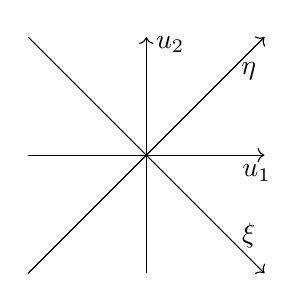
\begin{tikzpicture}
\draw[->] (-1.5,0) -- (1.5, 0);
\draw[->] (0,-1.5)-- (0,1.5);
\draw(1.4, 0) node[below]{$u_1$};
\draw(0, 1.4) node[right]{$u_2$};
\draw[->] (-1.5, -1.5) -- (1.5, 1.5);
\draw[->] (-1.5, 1.5) -- (1.5, -1.5);
\draw(1.3, 1.3) node[below]{$\eta$};
\draw(1.3, -1.3) node[above]{$\xi$};
\end{tikzpicture}
\]
\end{column}
\begin{column}{0.6\textwidth}
$\xi$成分だけでは、鏡映対称な運動しか記述できない。$\rightsquigarrow$
$2$次方程式で、係数$b,c$が$\sigma_{\alpha \beta}$対称なために解$\alpha,\beta$を
記述できないのと同じ。

$\sigma_{\alpha \beta}$で反転する$\alpha - \beta$によって
解が記述できたように、鏡映変換で反転する$\eta$成分によって
任意の(対称性から解放された)運動を記述できる。
\end{column}
\end{columns}
この$\xi$成分が重心座標、$\eta$成分が相対座標に対応している。
\end{frame}

\begin{frame}
\frametitle{系の持つ対称性}
$2$次元空間$\bm{u}$を$\clr{\xi, \eta}$で記述するのは、
要は座標変換(直交変換)である。

この座標変換が今の$2$質点連成振動子系と相性がいいのは、
運動方程式の係数行列$M$と、鏡映変換の行列$D$が交換可能
\begin{align}
D M = M D
\end{align}
だからである。

交換可能$\Leftrightarrow$同時対角化可能が効いて、
鏡映対称性による空間の分解(重心座標、相対座標)が、
運動方程式を解く上で有用になる。
\end{frame}

\begin{frame}
\frametitle{変換$\leftrightarrow$対称性}
鏡映対称性が、重心座標、相対座標への座標変換を導いたように、
空間の対称性と変換は強く対応している。

$N$質点の自由端連成振動子系では、鏡映対称性の他に
並進対称性$u_i \mapsto u_i' = u_{j+k}$があり、
この対称性がいわゆる離散Fourier変換を導く。
\end{frame}

\begin{frame}
\frametitle{対称性で空間を拡げる}
$2$質点連成振動子系では、最初に$2$次元空間$\bm{u}$を考えて
それを対称成分$\xi$と反対称成分$\eta$に分解した。

最初に対称な空間($=$自由度の低い空間)があり、
そこから対称性を破る方向に空間を``拡げる''という発想もあり得る。

例えば、任意のベクトルはある軸について$2\pi$回転すると元に
戻る($2\pi$回転対称)。\\
そこで「$2\pi$回転すると$-1$倍する」ようなものを考えて、
対称性を崩すことで出てきたのがスピノル(スピン)、という解釈もできる。
その背景には$SO(3)$と$SU(2)$という群がある。
\end{frame}

\begin{frame}
\frametitle{情報科学への応用}
例えば画像認識における機械学習において、augmentation として
回転変換や並進変換を行うことがある。

それらの変換(画像$\mapsto$画像)は、その画像のクラス(顔、猫、$\ldots$)を
変えないという点で``不変''性を誘導し得る。

その辺りから群論的考察ができる可能性はあるが、今のところ、
有用かつ見通しの良い理論は、誰も構築できていないようである。

機械学習の枠組みでは、入力データと予測結果の型(集合)が異なるため、
群論における変換との相性が悪い。\\
(すると、AutoEncoder のようなモデルは都合がいいのかも)
\end{frame}

\begin{frame}
\frametitle{まとめ}
\begin{enumerate}
\item 群とは変換を集めたもの。
\item 変換の裏には対称性があり、対称性は空間を分解する。
\item 群という視点で、空間を分解したり拡大したりできる。
\end{enumerate}
\end{frame}

\begin{frame}
\frametitle{参考文献}
\printbibliography
\end{frame}

\end{document}
%%% Local Variables:
%%% mode: latex
%%% TeX-master: t
%%% End:
